Poniższe wykresy przedstawiają liczbę aktywnych węzłów sieci w czasie oraz w zależności od rozmiaru pakietu i odstępie czasu pomiędzy kolejnymi pakietami. Sieć składała się z dwustu węzłów, które rozmieszczone zostały zgodnie z rozkładem normalnym. Różnice pomiędzy wariantami protokołu LEACH są mniej wyraźne niż w przypadku sieci składającej się z dwudziestu węzłów. Najwrażliwszym na zmiany parametrów symulacji protokołem okazał się LEACH DCHS. Sieć go używająca działa wyraźnie krócej od pozostałych wariantów krótszych okresów pomiędzy pakietami oraz nieznacznie dłużej dla dłuższych okresów pomiędzy pakietami. Czas działania sieci dla protokołów Flood i SPIN podobnie jak w poprzednio pozostaje niezmienny, niezależnie od dobranych parametów wykresu.

\begin{figure}[!htbp]
	\begin{center}
		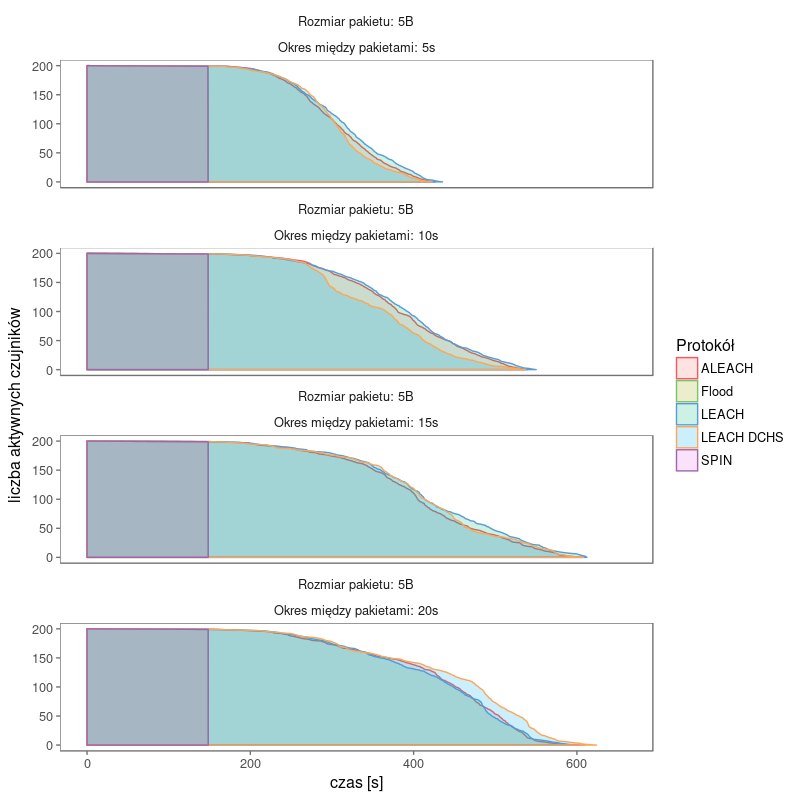
\includegraphics[scale=0.7]{\ImgPath/charts/alive_nodes_normal_200sensors_row1.png}
	\end{center}
	\caption{Aktywne węzły - 200 czujników, rozkład normalny, rozmiar pakietu: 5B}
\end{figure}

\begin{figure}[!htbp]
	\begin{center}
		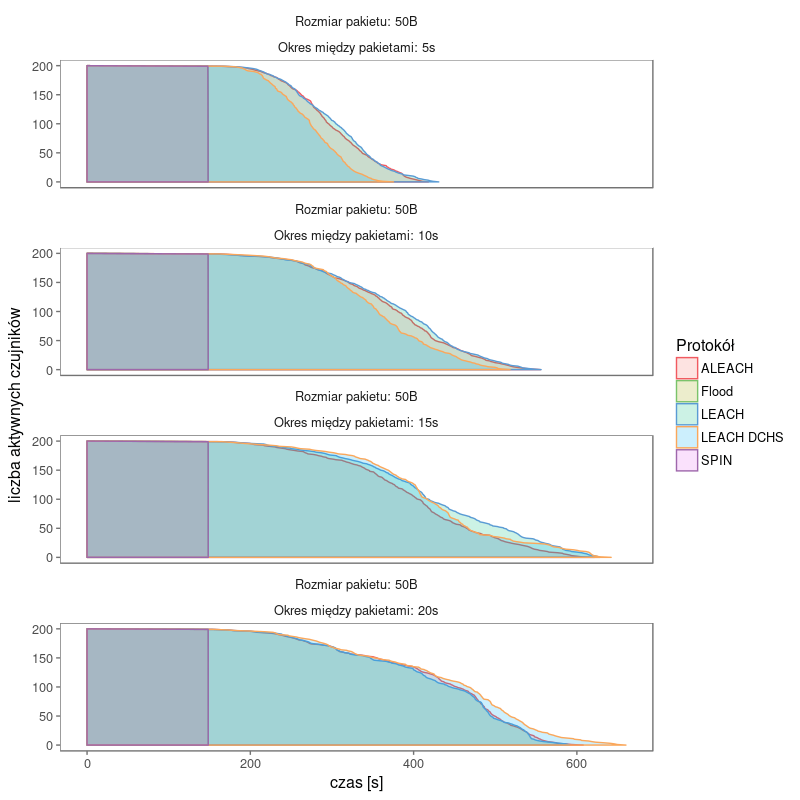
\includegraphics[scale=0.7]{\ImgPath/charts/alive_nodes_normal_200sensors_row2.png}
	\end{center}
	\caption{Aktywne węzły - 200 czujników, rozkład normalny, rozmiar pakietu: 50B}
\end{figure}

\begin{figure}[!htbp]
	\begin{center}
		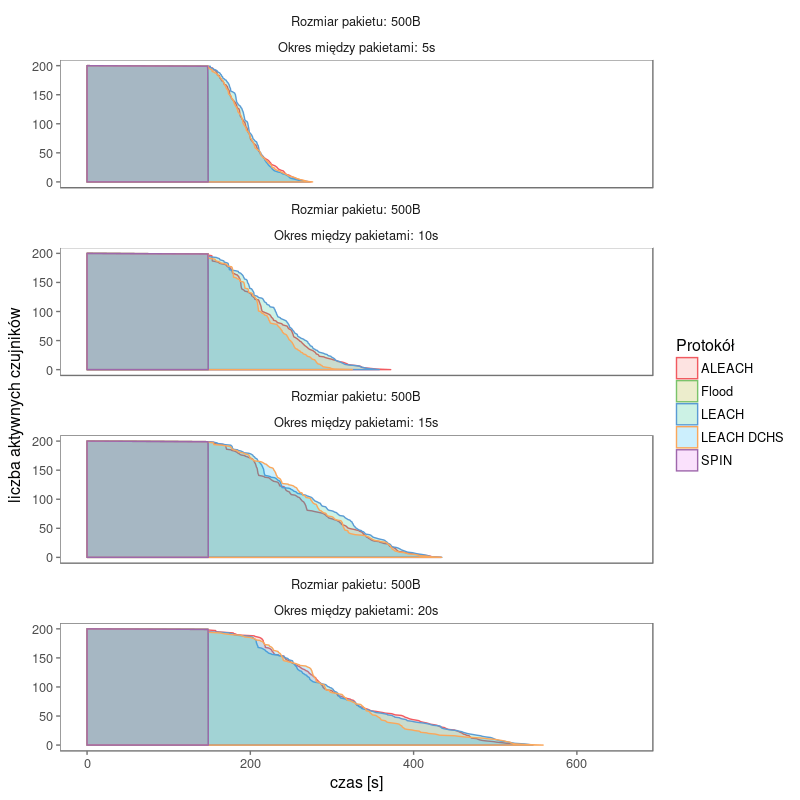
\includegraphics[scale=0.7]{\ImgPath/charts/alive_nodes_normal_200sensors_row3.png}
	\end{center}
	\caption{Aktywne węzły - 200 czujników, rozkład normalny, rozmiar pakietu: 500B}
\end{figure}

\begin{figure}[!htbp]
	\begin{center}
		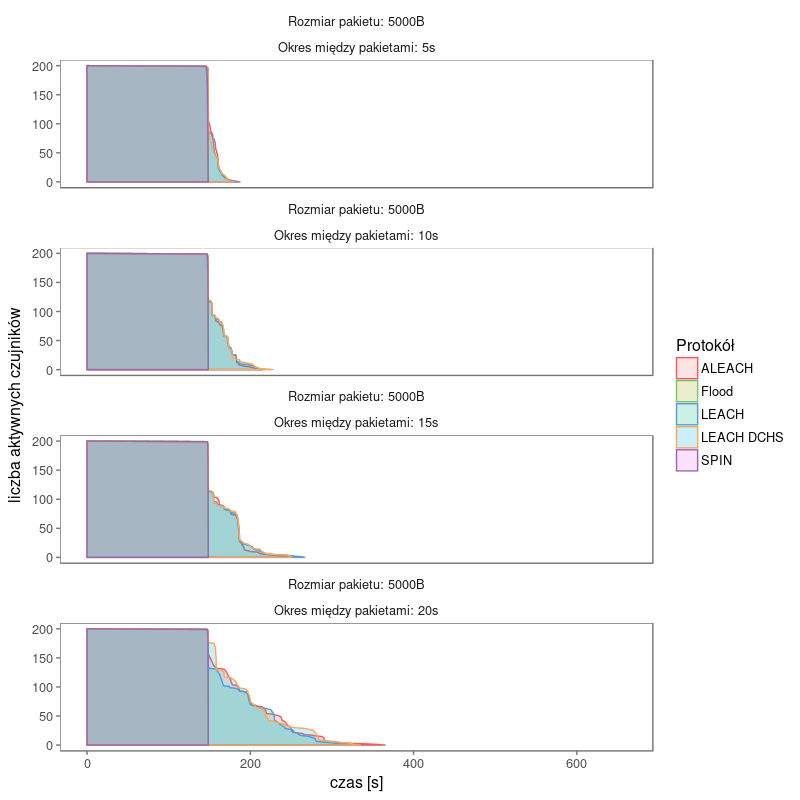
\includegraphics[scale=0.7]{\ImgPath/charts/alive_nodes_normal_200sensors_row4.png}
	\end{center}
	\caption{Aktywne węzły - 200 czujników, rozkład normalny, rozmiar pakietu: 5000B}
\end{figure}

\begin{figure}[!htbp]
	\begin{center}
		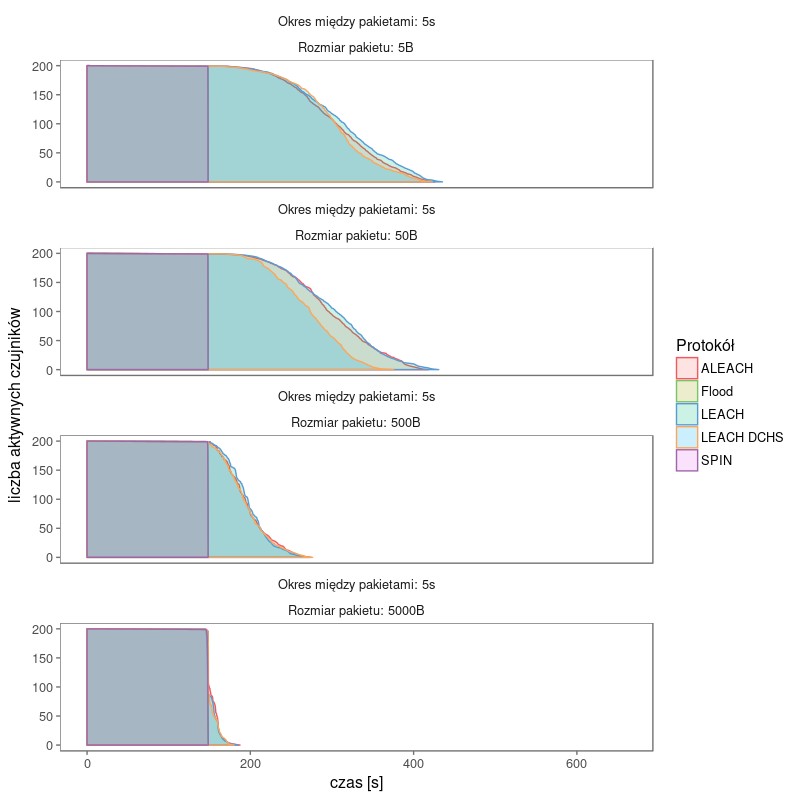
\includegraphics[scale=0.7]{\ImgPath/charts/alive_nodes_normal_200sensors_col1.png}
	\end{center}
	\caption{Aktywne węzły - 200 czujników, rozkład normalny, okres pomiędzy pakietami: 5s}
\end{figure}

\begin{figure}[!htbp]
	\begin{center}
		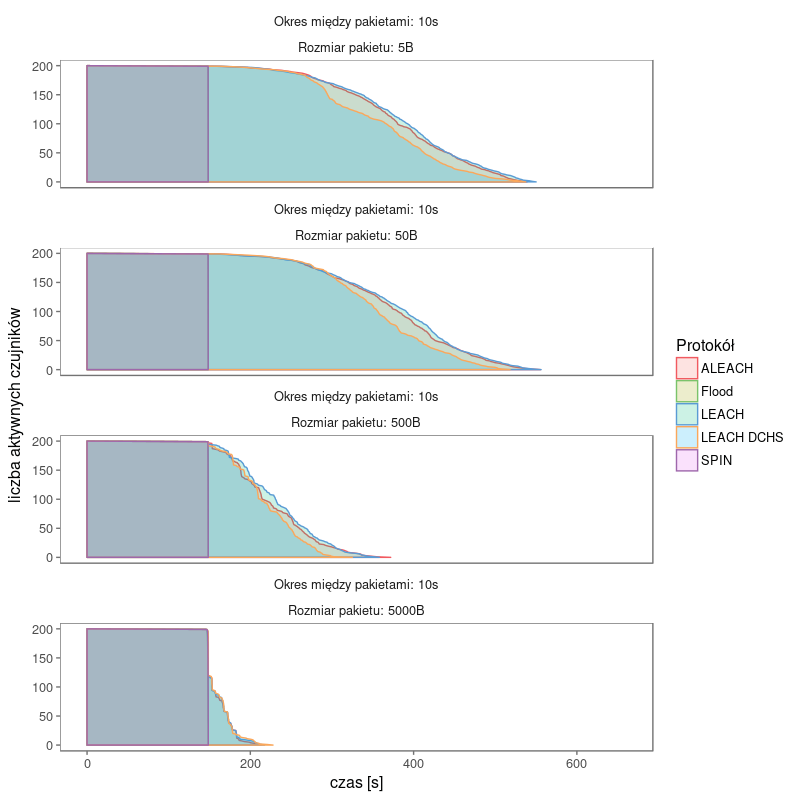
\includegraphics[scale=0.7]{\ImgPath/charts/alive_nodes_normal_200sensors_col2.png}
	\end{center}
	\caption{Aktywne węzły - 200 czujników, rozkład normalny, okres pomiędzy pakietami: 10s}
\end{figure}

\begin{figure}[!htbp]
	\begin{center}
		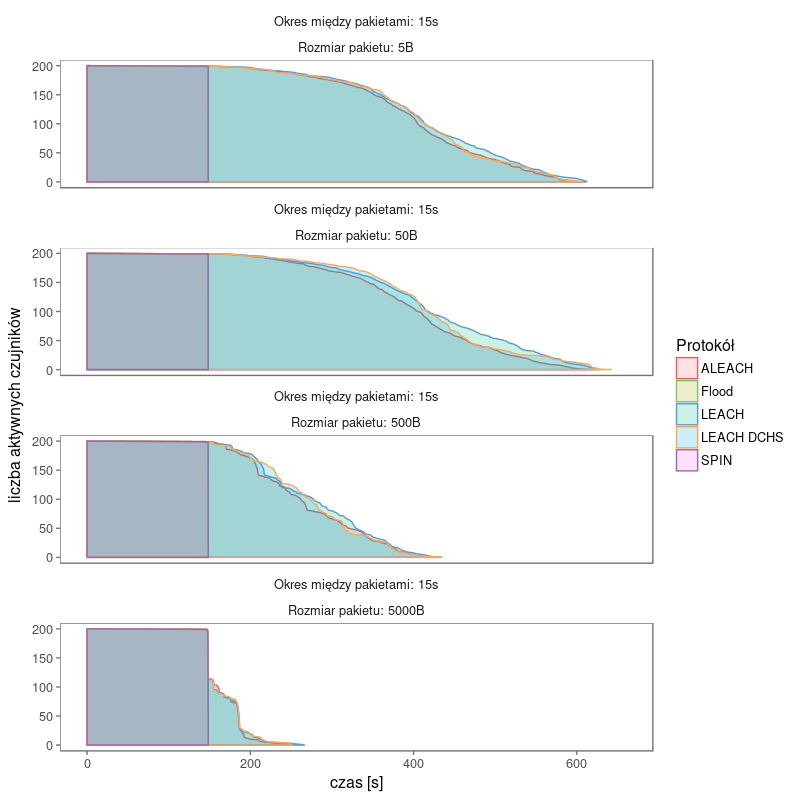
\includegraphics[scale=0.7]{\ImgPath/charts/alive_nodes_normal_200sensors_col3.png}
	\end{center}
	\caption{Aktywne węzły - 200 czujników, rozkład normalny, okres pomiędzy pakietami: 15s}
\end{figure}

\begin{figure}[!htbp]
	\begin{center}
		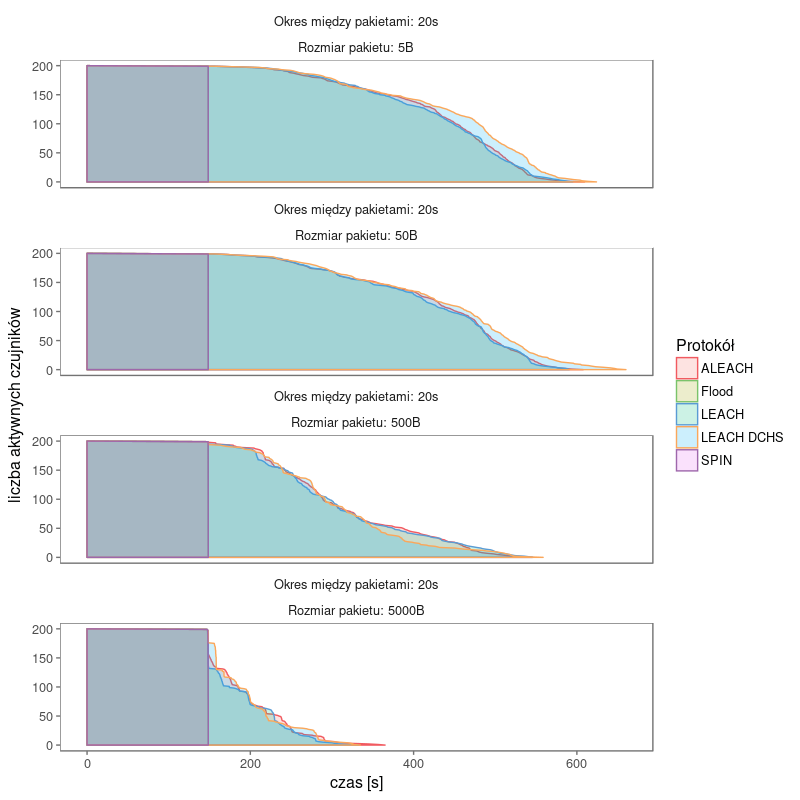
\includegraphics[scale=0.7]{\ImgPath/charts/alive_nodes_normal_200sensors_col4.png}
	\end{center}
	\caption{Aktywne węzły - 200 czujników, rozkład normalny, okres pomiędzy pakietami: 20s}
\end{figure}

\begin{figure}[!htbp]
	\begin{center}
		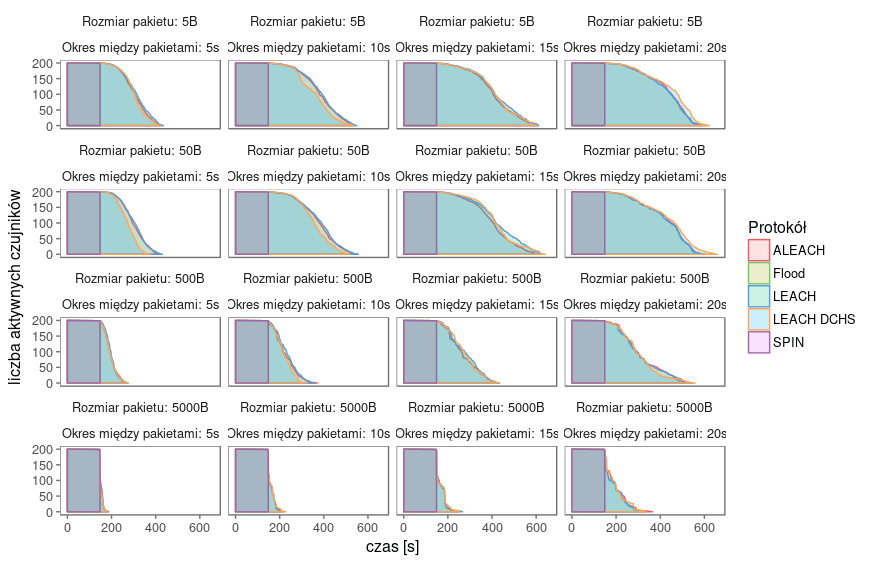
\includegraphics[scale=0.7]{\ImgPath/charts/alive_nodes_normal_200sensors.png}
	\end{center}
	\caption{Aktywne węzły - 200 czujników, rozkład normalny}
\end{figure}